\chapter{Trash in Culture and Theory}

% FROM Uncle Fernando’s Garbage Triptych, http://alphabet-city.org/issues/trash/articles/uncle-fernando-s-garbage-triptych, http://priscilauppal.ca/books/alphabet-city/
\epigraph{Anger is nothing compared to garbage:\\ Garbage eats anger for breakfast.\\ It eats all of us in the end.}{\hfill---Priscilla Uppal, \quotes{Uncle Fernando’s Garbage Triptych}}

In this chapter trash (and the practice of transforming trash) is examined in theoretical (and conceptual) aspect. Theoretical foundations of trash are discussed. (Further benefited from historical and social aspect of trash. (?)) How do scholars conceptualized the trash? What do they say about it? 

Trash draws attention of many scholars and people who are professional in different areas. Further trash is a common topic(problem?) of the all ages through the human history. In other words this topic is not introduced in recent years (or ages). It always part of the human practice and life. Even if trash is refused and discarded thing, there are people giving attention to them.


%%%
%%%
%%%
\section{Throw away culture}
We need to ask what is the source of trash.

Continuously consuming things and disposing of something. It is an important concept to understand why trash is trash? (or how it become trash?) Behavioral pattern of throw away culture results in the trash. (This pattern does not consider recycling of it.) Artworks that are trying to raise awareness is related with this concept.

(Our trash generating behavioral daily consumption patterns \ldots What are the results of them? Why are they throwing?) (There is a behavior that throws away and opposite of it there is a collecting behavior.) 

%%% Reference from Identity, mobility and the throwaway society
\todo{we live in a throwaway society (Barr, 2004; Cooper, 2003, 2005; Cooper and Mayers, 2000; Strasser, 1999, cf. O’Brien, 1999; Hawkins and Muecke, 2003); (ref from another article)}

\quotes{In the two previous sections we have demonstrated the paucity of the thesis of the throwaway society. In this thesis the undeniable matter of waste, itself pressing, urgent and excessive, is used to infer the presence of a society defined by its generation; a society ceaselessly discarding and abandoning its surplus as excess, as part of an endless desire for the new. Morally corrupt and unequivocally environmentally damaging, the rhetoric of the throwaway society classifies discarding as intrinsically bad and commands us to assume control of our wasting, suggesting the adoption of heightened regulatory practices around disposal as the means to ensure that we clean-up our act. The thesis, however, lacks depth and provenance. It is, actually, glib. Indeed, to infer the presence of a throwaway society from contemporary levels of waste generation is problematic for at least four reasons.}
% In this paper criticized the perception of throw away culture and arguments. They show the weak points of the arguments. What I understand from trow away culture?

In the scope of this thesis increasing consumption is motivator (draws attention more) but it does not bind to this. Always needed to keep in my mind that the practice of discard does not exist on only current societies. 

Life magazine fashionably heralded the advent of the "throwaway society" in 1955. 1971 daniel ingersoll reporting on his findings in the journal man in the notheast, "the industrial revolution ... was supplying the customer with hundereds of disposible containers and materials bt the end of the nineteenth century. the estimated 25.000 cubic yards of fill deposited in the upper portion of puddle dock show that the age of the throw away world began not in the twentieth century but during the nineteenth."

\todo{throw away sprit}

Industrial age played significant role (engine of the mountains of rubbish.)

% Resource is here: mmmacleo2005.pdf (throw away culture ile ilgili.) (Çünkü ben bunun ürününü kullanıyorum.)

% Çevremiz tek kullanımlıklarla dolmuş taşmış durumda, bu iki sanatçıda bunları anlatıyor.

% COFFEE CUP / Transforming them and invite other people, reveals its process.
% FROM http://www.gwynethleech.com/public-drawing/cup-windows/statement
  \begin{figure}[h!]
      \centering
      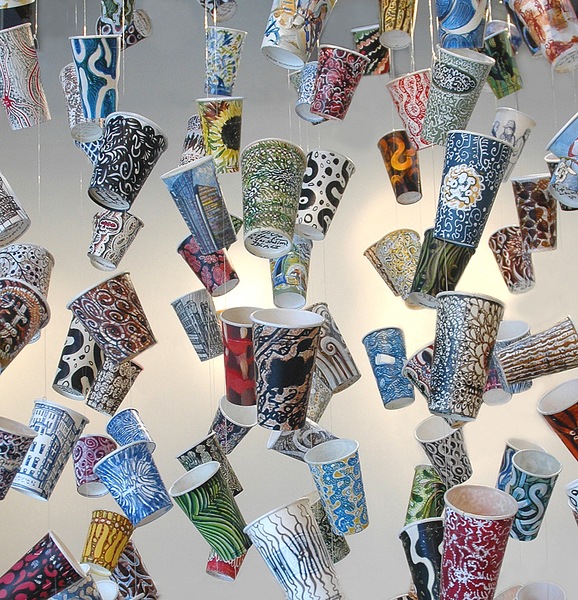
\includegraphics[width=0.5\textwidth]{graphics/Gwyneth-Leech-cup5.jpg}
      \caption[Gwyneth Leech, 365 A Year in Cups, 2013, Mixed media on upcycled paper coffee cups, Dimensions Variable]{I began to save all of my coffee cups to use as "canvases" for making art. Transforms coffee cups that are no longer trash but a vehicle for art, ideas, conversation and memories of a social moment upcycled from the detritus of our throw-away caffeine culture. I like my coffee or tea in a paper take-out cup. Even better than the contents, I like the used cup as a surface on which to draw and paint. And on the bottom of each one, I write the date, location, occasion and beverage consumed so that every hand-made cup artwork becomes the record of a social moment. For ArtPrize I am showing 1001 of my cup artworks, each representing a daily caffeine break. The installation makes visible largely unconscious patterns of consumption; this is what one simple take-away purchase looks like over the course of three years, this is what would usually be thrown away. It can be seen as a measure of time gone by, of money spent, of space to be taken up in a landfill. But as I upcycle each used cup into an artwork, it becomes the measure of other things as well: an artist's regular habit of generating new ideas, a diary of time spent with friends and colleagues, and the cumulative positive effect of doing something small and manageable every day.}
      \label{fig:GwynethLeech_TheCup}
  \end{figure}

  \begin{figure}[h!]
      \centering
      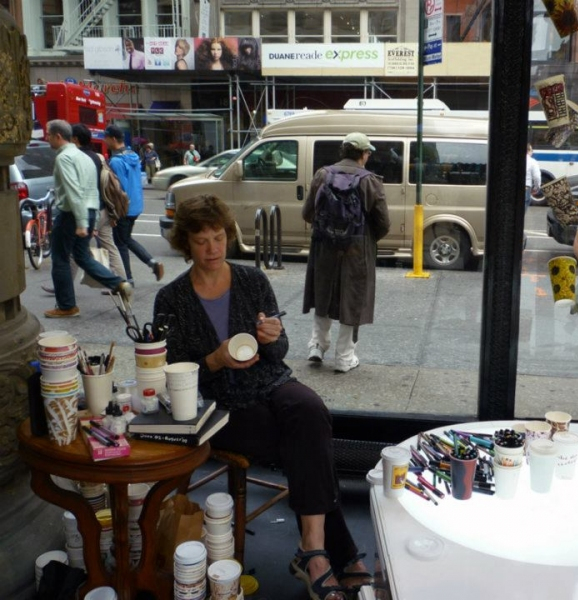
\includegraphics[width=0.5\textwidth]{graphics/Gwyneth-Leech-cup3.jpg}
      \caption[Gwyneth Leech while painting in the public]{There are different versions of it. paintings on paper coffee cups displayed as installation in public window spaces. She publicly draw their cups (the cup art window installation and public drawing project were on view repeated showed at many placas and date. During public drawing projects she draw with other people. and so. Buying a beverage is a daily event for Leech (and also many people. These coffee shops all around the world.}
      \label{fig:GwynethLeech_InAction}
  \end{figure}

% Günlük alışkanlıkların, dikkaten kaçan şeylerin aslında farklı şeylere dönüşmesini görüyoruz.

% TEA BAGS
% FROM https://instagram.com/silvirub/, http://www.rubysilvious.com/363-days-of-tea
  \begin{figure}[h!]
      \centering
      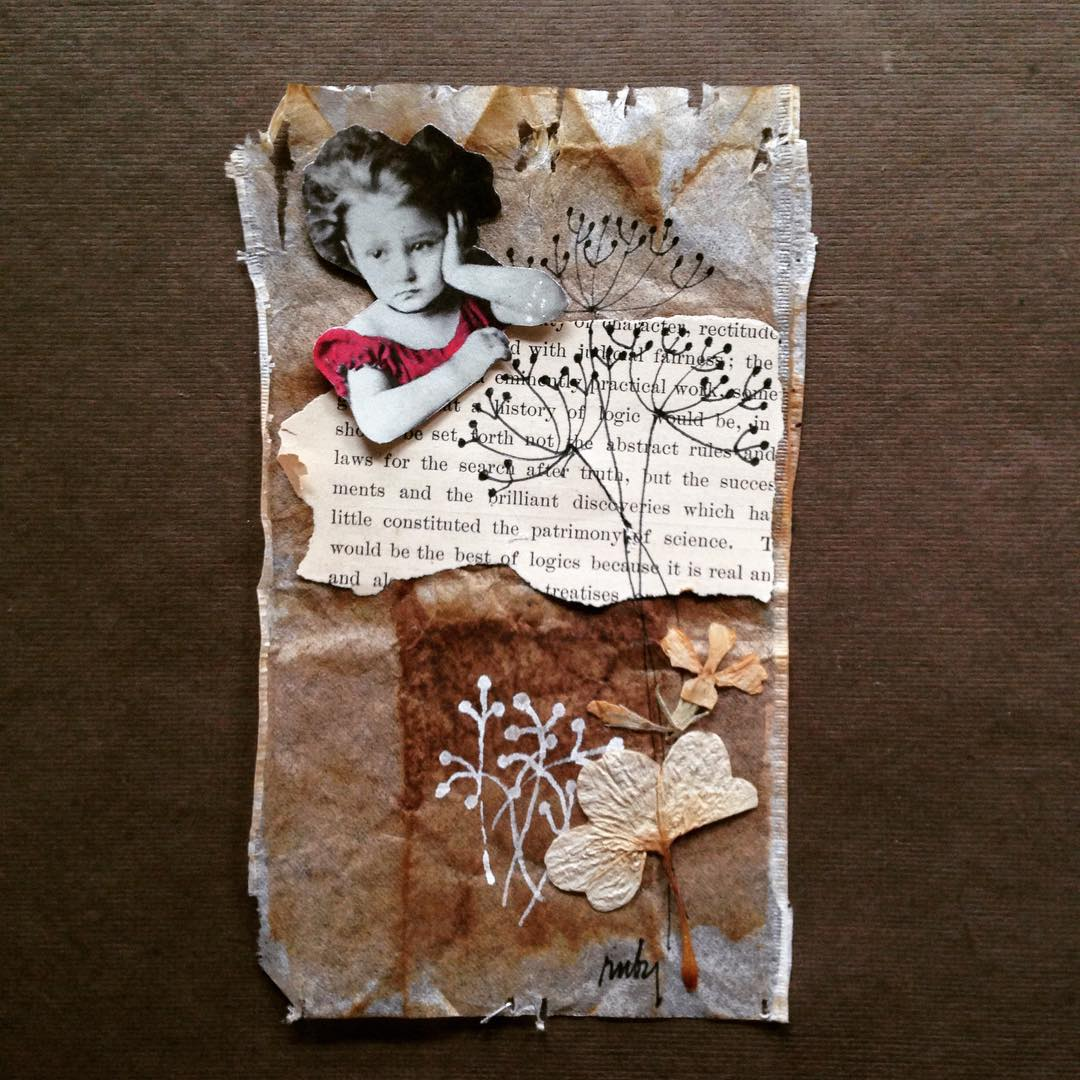
\includegraphics[width=0.5\textwidth]{graphics/rubysilvious-teabag-Day237.jpg}
      \caption[Ruby Silvious, 363 Days of Tea, Day 237, 2015, Mixed media on upcycled paper tea bags, Dimensions Variable]{In the beginning of this year, visual artist and graphic designer Ruby Silvious embarked on a quirky, personal experiment, set to last for 363 days. She decided to repurpose soggy and stained tea bags as unconventional, blank canvases, just waiting to be filled with her artistic expression. The project, entitled 363 Days of Tea, allows Silvious to challenge herself by transforming the recycled material with her intricate illustrations—the artist draws, paints, and forms collages on the salvaged tea bags. This project serves as Silvious’ daily journal, allowing her to record her thoughts and feelings by creating wonderful moody and whimsical designs on little teabag papers. Every day she creates a new piece that reflects her impressions in that moment. Currently based in New York, Silvious’ work has been exhibited internationally and she has received awards and recognition for her talents in paper work, print making and now her most recent endeavour of re-purposing recycled and found materials.}
      \label{fig:RubySilvious_TeaBag}
  \end{figure}

%****************************************
% Caps Seurat, 2011 60x90" in one panel, and 88x132" in 3 panels. Depicts 400,000 plastic bottle caps, equal to the average number of plastic bottles consumed in the United States every minute.

% Potraits of Global Mass culture from Chris Jordan. In Running the Numbers, photographer Chris Jordan attempts to convey the vastness of modern consumption by breaking down annual statistics into more graspable quantities depicted by clever visualizations made of individual objects or groups of objects that he photographs. “There’s a disconnect that happens when we assume we know what we’re talking about when we talk about hundreds of millions of plastic bottles,” Jordan says. “I’m trying to translate these numbers from the deadening language of statistics into a visual language that allows some kind of comprehension.”

% Many of Jordan's works are created from photographs of garbage and mass consumption Jordan uses everyday commonalities such as a plastic cup and defines the blind unawareness involved in American consumerism. His work, while often unsettling, is a bold message about unconscious behaviors in our everyday lives, leaving it to the viewer to draw conclusions about the inevitable consequences which will arise from our habits

% Bu adam çok güzel bir şekilde küresel tüketimi ve onun sonuçlarını anlatıyor.

% He recreates the most remarkable artworks with combining bits of trashes as a mosaic. Here he draw attention to the our consumerism and express them numbers that are very big to understand. All the material that we have is trash to create this pictures.

% Chris jordan hem bir gerçeği açığa çıkarıyor. 
% Diğerinde ise belki de anlamamızı sor kılan gerçerkleri çöple ilgili, bizimle ilgili olanları gene bizim önümüze sunuyor. Bize konuya farklı bir açıdan bakmaya davet ediyor.
%........................................


%****************************************
% HAKAN GÜRSU
% Buraya aslında bir de Hakan Gürsu koymak gerekli olabilir. Yani aslında kendisi pek de sanatla ilgili bir laf etmiyor. Ama aslında tükettiğimiz onlarca şeye karşı bir tavır yaklaşım sergiliyor. Bu yüzden theory kısmında yer alabilir. Bu çöpün içinde boğulacağımızdan bahsediyor. Onu dönüştürmek gerekliliğinden yeteneğinden bahsediyor.


% TEZ STATEMENT.
% Ya gerçekten çöpü dönüştürüyorlar ya da çöpe dair düşünceleri dönüştürüyorlar, ve bunu ele alırken aslında heykel, kolaj, fotoğraf gibi şeylerden yararlanıyorlar ama aslında ortaya koydukları şey bir sanatsal eylem. veya bunu sanatsal eylem bağlamında ele alabiliriz.

% Aslında şöyle bir şey var mustafa, aslında sanatçının yaptığı şey ürünlerinden çok tekrar ve devamlı olarak eyleme geçirdiği yaklaşımı. Çöpün de bu tekrar eden yapısı buna uyum sağlıyor. Çünkü zaten hatayın sürekli bir parçası. Aslında bunun için şart olmasada destekleyici olduğu söylenebilir.
%........................................


%****************************************
% Tracy emin mesela. Yani aslında bir şekilde bir yandan aslında teoriye mi değiniyorum yoksa sanatçıların işlerine mi değiniyorum, bunların teorideki karşılıklarını mı buluyorum emin olamadım. Bunların ikisi paslaşarak ilerliyor aslında. Aslında çöplerin bize ait çok şeyler söylediğini ünlülerin çöplerini karıştıran yaklaşım ortaya çıkarıyor. Bu işde bununla ilgili aslında.
%........................................


%%%
%%%
%%%
% FROM Examined Life
\section{Zizek's Approach to Garbage}
(There is a curious fragment where Zizek, dressed as a sanitation man, stands in a waste deposit in a pile of garbage and ponders over garbage and human existence. In documentary film, Examined-life, Zizek talks about ecology in the middle of a garbage dump in London, and his part starts with these sentence: "This---garbage dump--- is where we should start feeling at home". He asserts his claim at first and go through explaining how ecology turns to ideology and mentions wrong perception about the ecology. Draw attention to notion of even if trash disappears from our world but not world. It seems as though the thrown out garbage disappears from our world. However, it disappears only from the world of illusions, but still exists in reality. He thinks that the way of approaching ecology is problematic, because accepting that nature as a balanced harmonious thing. He claims that it is ideological in the sense that wrong thinking important problems. Nature contains unimaginable catastrophes. think oil and distinct animals and plants. we profit balance part of the nature but it is created from catastrophe. Are we aware of this catastrophe. He asserts that ecology will slowly turn to religion that "is a kind of an unquestionable highest authority." Ideology of ecology warns us like, "Don't do that. It would be too much." its voice is like "Don't mess with D.N.A. Don't mess with nature. Don't do it" etc. We should not forget that we are part of the ecology. We must more alienated from the nature. We must find poetry and spirituality in the dimension of trash. That's the true love of world. Love is not about idealization. This part will be extended later.)

% FROM https://commons.wikimedia.org/wiki/File:Albatross_at_Midway_Atoll_Refuge_%288080507529%29.jpg
  \begin{figure}[h!]
      \centering
      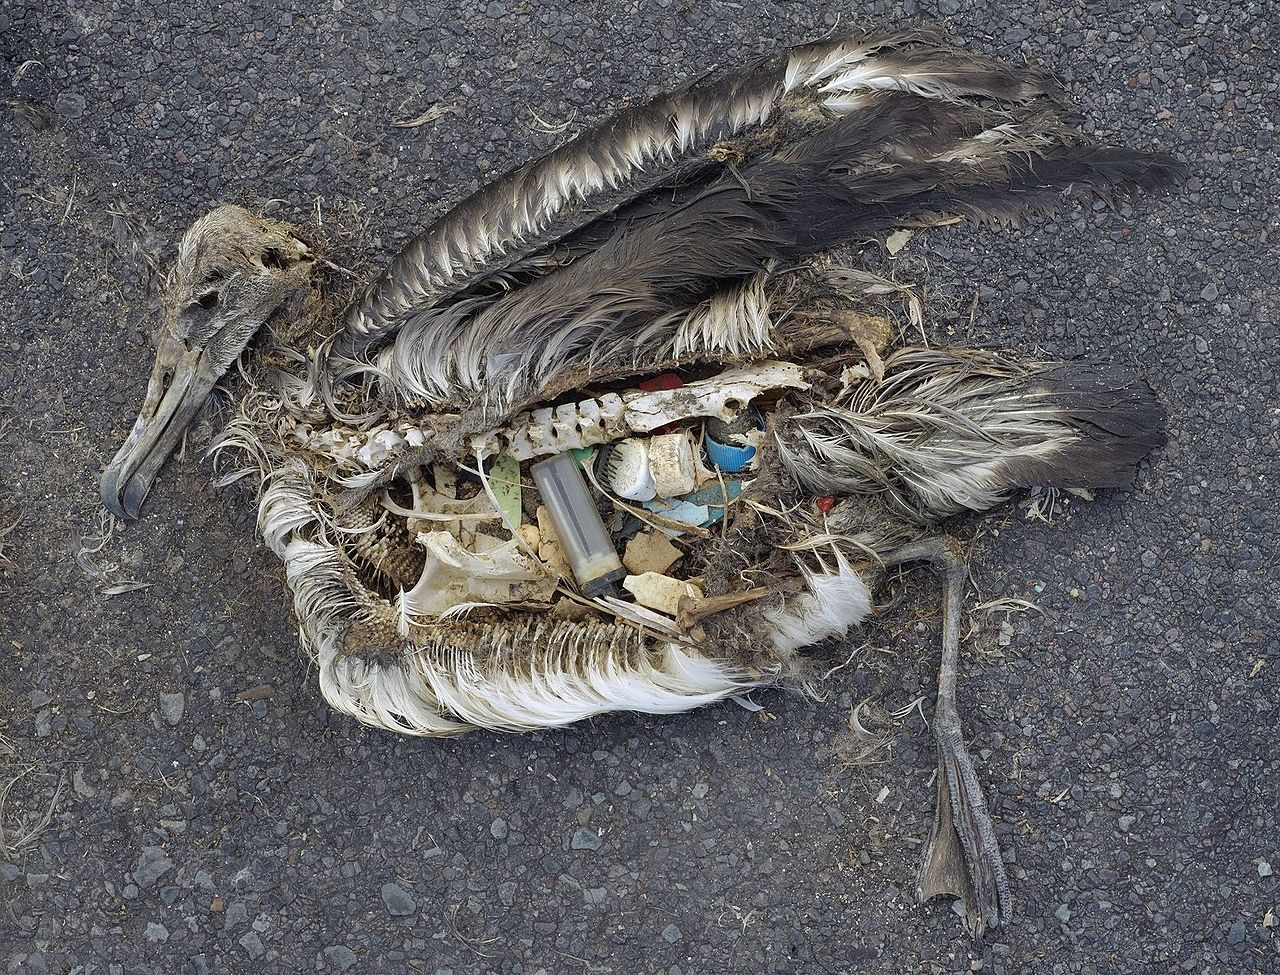
\includegraphics[width=0.5\textwidth]{graphics/ChrisJordan-Albatross.jpg}
      \caption[Chris Jordan, Albatross at Midway Atoll Refuge, 2009]{The unaltered stomach contents of a dead albatross chick photographed on Midway Atoll National Wildlife Refuge in the Pacific in September 2009 include plastic marine debris fed the chick by its parents.}
      \label{fig:ChrisJordan_Albatross}
  \end{figure}

Using spare narration and stunning imagery, Chris Jordan's feature film MIDWAY explores the plight of Laysan albatross plagued by the ingestion of our plastic trash. Both elegy and warning, the film explores the interconnectedness of species, with the albatross on Midway as a mirror of our humanity.

Even if garbage leave outs our life, we do not care about the results of it. And it is captured by the works of Chris Jordan.In this photo series it captures 


% Effect of plastic on wildlife in Antartica.
% Her ne kadar biz çöpü attıktan bizim hayatımızdan çıksa da yok olmuyor. Sadece başka bir yerlere gidiyor. Mesela kuşların midelerine. Chris Jordan'ının imageları bunu çok da güzel açığa çıkartıyor. Bizim çöpleriminde habersiz hayvanlar bunları yiyorlar. Bir yandan ürettiğimiz ürünler ile kaynakları tüketirken bir diğer yandan ise artıklarımız diğer yaşanları tüketiyor. Dikkat çekmek istediğim nokta aslında ekolojik hassasiyetlerden çok aslında elimizde avucumuzda ne varsa onları tüketiyor olmamız. Karşı durduğum nokta ise tam olarak burası. 


\quotes{According to Zizek, modern understanding of ecology is the real false consciousness, connected with mystification of real problems. Postmodern mysticism arises when disasters begin to be rationalized, interpreted in strict logic terms of cause-effect relations. Such interpretation makes life easier. However, nature is not an absolute balance and total harmony (this aspect of Zizek’s thought makes him akin to classical conservatives). Nature is a series of unthinkable disasters. Zizek believes that ecology is transforming into a new western conservative ideology: “One should not play games with nature! Do not touch DNA! Do not develop new medicines! Do not invent new technologies!” How one should react to these reproaches? Zizek’s recipe is to reinforce alienation from nature, to become more artificial.} \cite{vafin2012zizek}

His basic argument is that the modern eco movement is a conservative ideology. It says don't do X from an authoritarian high ground and it idolizes and mystifies ecology. Basically he says the eco movement has it's head in the clouds. If it loved the environment it would recognize the rubbish we create and the chaotic nature of ecological change and try to further divorce itself from that process(nature) and try to turn the whole thing into art. 

\begin{itemize}
\item Our relation to our filth follows an “out of sight, out of mind” principle, but trash doesn’t disappear.
\item Ideology addresses real problems but mystifies them.
\item We search for meaning when a horrible event happens to make it easier to accept.
\item The ideology of ecology is that world is in the best possible state and that humans disturb nature.
\item Nature is not an organism in balance that humans exploit, but rather a series of great catastrophes.
\item Ecology is becoming more like religion with dogmas.
\item Even if we learn the potential catastrophes of nature, we ignore them as long as they don’t manifest near us.
\item The solution is not to worry about saving nature, but to figure out how to survive without it by becoming more artificial.
\item Learn to love our trash as a part of ecology.
\end{itemize}	

How much harmonious all these produced materials with nature? How many animals and the plant can use these discarded items? (Because of complex production methods their recycling requires complex processes again. Some of them already produced to protect goods from natural factors (like decaying etc.). However how can we protect nature from them?) It is very hard that spontaneously they become harmonious with nature. However, some artists turned to trash into site-specific sculptures that are more than trash heap. not discarding but bracing our attitudes turned them to a something that worth it to watch and think about it. (Converting what we create harmonious with the existing system.) Because it is not possible to think that nature will live harmoniously what we created. The more likely idea will be we will live harmoniously with what we create.

Getting rid of it is not the significant action. It still waits us at somewhere else or the next generations have to cope with it. (Establish relationship with the afterthought.) Maybe the first thing to do is accept the trash, to accept that there are things out there that serve nothing. To break out of this eternal cycle of functioning.

The issue of trash is not limited with ecological and economic perspective, it has also other dimensions.(draw attention to multidimensionality of this topic, but why? and what are the other dimensions?)

Trash itself is not the only problem, the practice, lifestyle causing it is more important problem. The dynamics of market and flow of objects into it plays important role production of trash.

Trash of developed societies has higher decomposing period in the nature. Therefore results in higher damage to the nature, hard to reuse, hard to transform, sometimes not to safe to keep them because toxic elements etc. 

\textbf{Summary.} Zizek mentions that ecology is something wrong point to approach this topic. Show the problematic understanding thought to the garbage. Suggest another thing, and point out the need for the new approach. Beyond the ecological problem there are different sides of it. Different readings can be added to the topic. Adding spirituality and new aesthetics dimension to the topic. 

% Her şey çöpe dönüyor. 
% En fazla ürettiğimiz şey çöp. Böyle giderse her şey her yer çöp olur mu? Aslında tezin konusu bu değil ve buna cevap verilmeyecektir? Ama WALL_E denilen dizi böyle bir alternatifte geçen bir dizi.
% İki tane yöntem var birisi bu çöp dağları... ve dağlardan ne görüleceği. Gerçi vik munizde o dağlara gidenlerden birisi ve oradaki insanlardan portreler yapıyor. Çöp dağlarını nasıl görmek gerek, nasıl farklı bir şekilde görebiliriz.
\comment{Zizekin çizdiği potreden aslında çöp dağlarınan oluşan bir dünya tasavvur edebiliriz. Ve bun noktada wall-e'ye bakabiliriz. Bir an için çöpümüzün içinde buğulacağımızı düşünürüz. Ya da bu çöp dağlarının bizleri sınırladığını düşünebiliriz.}

\comment{WALL-E belki olabilir. Dünyanın aslında bir çöp yığını haline gelmesini gösteriyor olabilir. Çöp dağları, çöp denizleri. Atılmış binbir türlü nesne. ve wall-e ise bunları ne yapıyor sadece pressleyip bir kenera bırakıyor. Bundan basetmişken aslında pressleme işi yapan şu cesar. Bu şekilde olmak zorunda mı? Bunun alternatifi yok mu? Aslında bu tezde bunlara cevap bulunabilir. Çöpe olan bir sürü yaklaşıma ek olarak bir de bunlar var. Ya da başka neler var? Bunları araştıran inceleyen bir yazı. Wall-E'nin çizdiği portreyi tekrar ele alırsak ne görürürüz. İnsanlık buna mı dönüşücek? Başka bir ihtimal yok mu? Gerçekten de dünyayı bekleyen şey bu mu? Bir çöp yığını olması mı? Bu bir abartı mı yoksa gerçeklik payı yadsınacak cinsten mi?}

\comment{WALL-E is a 2008 American computer-animated science fiction comedy film produced by Pixar Animation Studios. A robot named WALL-E, who is designed to clean up an abandoned, waste-covered Earth far in the future. WALL-E resembles giant dozers that moves and piles trash in the landfills. This robot creates squeezed trash blocks that have no meaning and interpretation. All different objects in terms of their physical and social properties turned to same squeezed garbage blocks. There are mountains of trash and place is very limited. By squeezing them, WALL-E saves space. \todo{What is the context of it? Which part is related with my topic?} What are we going to do with all these mountains of trash? \todo{Can it be placed under zizek part?} WALL-E represents a possible future condition of Earth.}

% HERŞEY ÇÖPE DÖNÜYOR. Relationship between entropy (second law of thermodynamics) and waste. Resources of nature turns to waste that it can revert it. Creating that are reversible again is problematic through the nature of sustainability. What is produced after it is consumed become worthless.

% Yani bir çözüm bulmaktan bahsediliyor ama sanat çözüm bulur mu bilmiyorum. Zaten derdim de benim aslında tüm bu çöp sorununu ele almak çözmek değil. Çöpe olan bakış açısındaki problemi göstermek olabilir. Burda beni destekleyen şey zizekin sözleri olacak.

idealization of nature, to love nature is to love trash. Live with trash. Do not see it as trash actually. Then the question is how to love trash? how to live with trash? can living with our trash enrich (our perceptions, abilities)? how not to see them as trash and useless? Can it be possible with art?

%%%
%%%
%%%
\section{Rubbish Theory}
Objects have a lifetime and they don't remain same through that lifetime. Their value, usage, location change over time. During its lifetime objects may circulate different markets and values systems like economical value, social value, aesthetic value etc. Especially this cycle has picked up speed with the advent of consumer culture, our most recent technological gadgets becoming obsolete within 3 years. Objects function and value are transformed by relocation and revaluation of objects from one place to the other or one discipline to another. This flow(transition) and transformation theorized with Rubbish Theory by Thompson \cite{thompson1979rubbish}. Thompson looks at the creation and destruction of value in man-made objects, cultural artifacts, and ideas. He notes how an object’s economic and/or cultural value diminishes over time rendering the objects worthless or redundant. The theory looks at how some of these objects then regain value, such as antiques or historic homes. It claims that there are three types of objects; transient (normal state, decreasing value, circulating), durable (permanent, increasing value, removed from circulation) and rubbish(zero value, will be destroyed or reinvested for economic and social value). The transition from transient to durable is only possible firstly transient to rubbish and later rubbish to durable. Further, there is a common idea/argument/motto that is "trash to treasure" among artists who use trash as a medium. Rubbish theory presents a conceptual approach to this argument. 

Although Thompson is quite successful categorizing states of objects throughout their lifetime, claimed transitions between states in the theory have some problems. Thompson label some transitions as possible and the others as impossible. "He allows goods only to move from a transient to become rubbish, and from rubbish they can either be destroyed or become durable. Movement in the other direction, from durable to either transient or rubbish, is not allowed in this system" \cite{meadow2011relocation}. Further, he does not allow move from transient to durable. However, Duchamp's fountain breaks this rule. Because urine used as a fountain is still functional and have a place in the market. In another word, it is not rubbish. This urine with the approach of Duchamp turned to be an artwork. It is one of the most influential piece of modern art and one of the best examples of ready-made. After Duchamp's intervention to the urine, it becomes a durable object placed in a museum.

In rubbish theory beyond the objects states how it happens transition of objects in practice is missing and Parsons fills this gap by claiming that transition from rubbish to durable are possible with finding objects, displaying objects, re-using objects \cite{parsons2008thompsons}. (explain details) (It can also be thought that they are the way of value creation.) (turning trash to treasure or something else is a value problem. transforming them creates new a value system? or just finding place existing value system. by the way there is a value theory related with (or inside of) game theory.)

Further another conducted research examines the psychological, social, and aesthetic factors involved in found object and found that ... \cite{camic2010trashed}.

"Rubbish theory, a philosophy that attempts to address how value is placed on material objects." "It is a body of thought that addresses how the value of material objects is socially constructed and deconstructed." "An awareness of rubbish theory is important to the understanding of the sociology of consumption and waste because, while what is and is not considered garbage may seem obvious and natural, the value of objects is based on the perceptions of people." "The classic examples of these categories are the durable 18th century Queen Anne tall-boy chest and the transient used automobile." "What decides whether or not something is a durable or transient is often the perceptions of the powerful members of society, those with a vested interest in owning objects whose value will always increase, while the remainder of society owns objects whose value will eventually decrease to nothing."

The paper suggests the Theory is useful in foregrounding the material dimensions of markets. It also highlights the importance of thinking in terms of movement, flow and circulation in markets. Finally the theory suggests that value emerges through our ways of seeing and placing objects. (From Liz Parsons)

%%
%%
\subsection{Rubbish Theory in Practice}
% TODO PRAP. REF.
(Summary From Liz Parsons.) 

A key critique of the rubbish theory is its neglect of the practices of value creation. Thus the paper draws from existing studies in consumer research in exploring three such sets of practices: finding objects, displaying objects, and transforming and re-using objects.

Plenty of work in consumer research explores the ways in which goods might act as symbolic resources for lifestyle and identity construction (i.e. Belk 1988), but there is less reflection on the actual practices and activities through which goods become meaningful and valued. McCracken’s (1988) work on ‘Meaning Manufacture and Movement in the World of Goods’ begins to address this gap. He views advertising and the fashion system as instruments of meaning transfer between the culturally constituted world and consumer goods. He then suggests that a series of consumer rituals operate to transfer meanings from consumer goods to the individual consumer. These rituals include those of possession, exchange, grooming and divestment. The strengths of his argument include a focus on the mobile quality of meaning and some exploration of the instruments though which meaning is transferred. However he is not clear as to the practices which constitute these rituals. In addition his contention that ‘meaning resides in three locations: the culturally constituted world, the consumer good, and the individual consumer’ (1988: 89) fails to completely capture the complexity and fluidity of meaning movement. There is a linearity to his conceptualisation which misses the constant flux and flow of meanings in markets.

In ‘The Social Life of Things’ Appadurai (1986) highlights the restlessness of objects arguing that ‘from a methodological point of view it is things-in-motion that illuminate their human and social context.’ (1986: 5). Appadurai usefully observes that ‘commodities, like persons, have social lives’ (1986: 3). He focuses on the ‘commodity potential’ of things. ‘things can move in and out of the commodity state, that such movements can be slow or fast, reversible or terminal, normative or deviant’ (1986: 13). However these movements do appear to be reduced to the opposites of commoditization and singularization, one might ask the question, does anything exist in-between? This is where Thompson’s Rubbish Theory comes in.

\subsubsection{Transients, Rubbish and Durables}
The category of objects and experiences of no value (rubbish objects and experiences) is largely invisible. The transient represents the usual state of commodities as objects which are declining in value and which have finite life spans. Whereas the durable increase in value over time and have (ideally) infinite life spans (1979: 7). Thompson uses the example of a used car as a transient and Queen Anne tallboy as a durable. He further observes that their category membership determines the way we act towards them. 

Thompson argues that rubbish represents an important possible ‘in-between’ category in a ‘region of flexibility’ which is not subject to the same control mechanisms of the valuable and socially significant categories of transient and durable. Therefore it ‘is able to provide the path for the seemingly impossible transfer of an object from transience to durability’ (1979: 9) he further suggests that ‘a transient object gradually declining in value and in expected life-span may slide across into rubbish’ (1979: 9) where it has the chance of being re-discovered, brought to light or cherished once gain. Figure one demonstrates the possible paths an object may take (from transient to rubbish and from rubbish to durable). 

Thompson comments that we only notice rubbish when it is in the wrong place, and highlights the embarrassment and anxiety that mis-placed rubbish, or rubbish which has found its way in to the wrong place can cause ‘Something which has been discarded, but never threatens to intrude, does not worry us at all.’ (1979: 92) but rubbish in the wrong place is ‘emphatically visible and extremely embarrassing’ (1972: 92). (Further there is similar analogy at Waste and Want. The author give the example of shoe and claim that thrash is relative. The shoe on the dinner table is something disgusting but in the foots is not at like that.) Rubbish objects are things that are no longer used or loved or cared for and often no longer seen. Rubbish objects linger on the periphery of our lives, in the back of the drawer, bottom of the wardrobe or cupboard, corner of the garage or garden shed gathering dust.

\quotes{In an ideal world\ldots an object would reach zero value and zero expected life-span at the same instant, and then... disappear into dust. But, in reality, it usually does not do this; it just continues to exist in a timeless and valueless limbo, where, at some later date (if it has not by that time turned, or been made, into dust) it has the chance of being discovered’ (1979: 8-9)}

\subsubsection{The Practices of Value Creation: From Rubbish to Durable}
Three such sets of practices are explored below, they include: finding objects, displaying objects and transforming and re-using objects. It is argued that each of these sets of practices changes the way we view an object moving it from being seen as a ‘rubbish object’ of no value to a ‘durable object’ of increasing value.

\textbf{Finding Objects:} One key way in which objects may slide from the category of rubbish to durable is through the act of finding. Indeed, Gabriel and Lang (1995) include the ‘Consumer as Explorer’ as one of many possible consumer identities.What, then might one mean by ‘the find’? Ultimately the find relates to discovery, and suggests that something has been otherwise overlooked, ignored or hidden away. The find may not involve objects which are new to us, it is possible to find some of ones own items if they have been hidden away long enough in an attic and thus made strange to us. The concept of the find also suggests that the found object has some qualities that others (or indeed ourselves) have in the past overlooked, as such it is closely related to ‘bringing to light’. The find may be extended to embrace features of objects as well as objects themselves. This directs us to their ‘potentialities’, objects may have been there all along but we’ve suddenly found them to be useful, likeable or beautiful. It might be that some aspect of them has simply been brought to our attention. Equally, as discussed below in relation to transforming objects, we may make alterations to objects which bring out their potential. The transition from thing of little or no value (rubbish), to thing of value (durable) can result form a relatively minor shift in the way we see something.

\textbf{Displaying Objects:} by displaying objects in home, fashion etc. (This is not a strong category.)

\textbf{Transforming and Re-using Objects:} These transformations may involve creating new uses for old things to fit in with contemporary lifestyles. Transformations may also involve the modification or updating of objects through painting, alteration or repair. Transformations may not only be based around creating new uses but also creating new looks. The re-use of objects also creates value for things that otherwise would be allowed to slip away (or slide terminally into the rubbish category).

%%
%%
\subsection{Theoretical Analysis of Found Object}
(Summary From Paul M Camic.) 

% TODO PRAP. REF.
\subsubsection{Seeking Objects}
As a species Homo sapiens has been gathering and collecting objects for thousands of years. Food, clothing, weapons, fuel, animals, and plants are the more obvious items, but visually pleasing objects, things that arouse curiosity, and shapes that stimulate the imagination have also been sought. The search for “things,” collecting them (Humphrey, 1979), and the need to embellish and make the ordinary special (Dissanayake, 1988) have been essential parts of the evolutionary process of human development (Bettinger, 1991; Dissanayake, 1992). For example, many early cave drawings occur around a natural feature within the cave such as a projection or indentation (Bahn, 1998; Lewis-Williams, 2004), making these natural features potentially comparable to found objects in modern and contemporary art (Read, 1930). When early prehistoric eople recognized a cave’s natural feature as a “found object” and incorporated it in a picture, it is possible that the natural feature took on a higher value than if left alone, thus adding to the value of the object on the cave wall. Once found and incorporated in paintings and drawings on a cave wall, it is possible that these protrusions and indentations became objects that functioned symbolically.

In contemporary societies, people seek objects to adorn bodies, decorate homes and gardens, and personalize places of work (Menzel, 1994). Seeking and finding objects, whether in vast Asian cities, remote African villages, or the high streets of Europe and North America, have become part of daily life for millions of people. Although most of these objects are purchased new in shops or online, many others are preused items, castoffs, or trash found in back alleys and country lanes, dumpsters, and rubbish bins or purchased cheaply in flea markets, garage and boot sales, and in shops catering in previously owned goods. Some individuals have chosen to salvage objects out of economic necessity, as depicted in Jean-Francois Millet’s 1857 painting The Gleaners and by Agne`s Verga’s 2002 documentary film Les Glaneurs et la glaneuse, whereas others have done it for a range of other reasons, including a desire to rescue them (Belk, Wallendorf, \& Sherry, 1989). These “other reasons” pose an opportunity for researchers to better understand why people voluntarily seek society’s discarded material objects and how they make use of them. A form of cultural reuse, the process
of salvaging and using found and second-hand objects has potential implications for \ldots 

% [TODO adapt for my case] The main aim of the current study was to produce an initial conceptual model that explains contemporary found and second-hand object use in blablabla.

% [TODO adapt for my case] Found objects first came to the attention of the general public through their use by artists in early part of the 20th century. To help contextualize the application of found objects, the following section provides an overview of their use by Western artists. This is followed by an examination of objects in human development and includes aspects of psychoanalytic theory, material objects and their relationship to identity, selected cognitive theories, and an outline of the social life of objects through rubbish theory.

\subsubsection{Found Objects in Art}
The term found object, as used in this article, refers to an existing object or artifact that is picked up (found) and generally not bought or originally intended as art, yet it is also considered to have some value (e.g., aesthetic, novelty, remembrance) to the finder. It is during the locating and finding process that the value of the object, once considered to be junk or rubbish, changes. The junk object becomes transformed into the valued found object. Objet trouve, translated from the French as “object found,” appears to have been first used by Marcel Duchamp in 1913 in reference to objects he made use of in his “readymade” art (Richter, 1965). His earliest known application for an objet trouve was seen in his well-known piece Bicycle Wheel, “where he had simply upturned a wheel on a stool” (Gale, 1997, p. 97) and labeled it a work of art. A more public and controversial introduction of the readymade occurred in 1917 when Duchamp attempted but failed to exhibit the highly contentious piece The Fountain, where a single white urinal became a readymade piece of art (Tomkins, 1996). These pieces were the beginning of Duchamp’s shift from an art striving for beauty and possessing a higher complex or hidden meaning beyond what was seen to an art form that made use of, and occasionally celebrated, the common materials and objects found in everyday living.

Gascoygne (1936), writing about the artist’s use of “the strange medley of materials” (p. 169), referred to as objets trouve in Surrealist art, suggesting that the artist “discovers a hidden symbolic significance in the [found] object which is preserved when the object is ‘framed’ as art” (p. 170). The finder discovers an unrealised significance in the object. A new boundary is formed around the object by the finder through removing it from its found environment and placing it in a new one, thus empowering the finder in the role of creating a new reality for the object. He argued that the found object, before it is found, approximates a zero value aesthetically; the zero value increases for the finder---beholder on discovery of the object and increases further if the object is placed in another context. \ldots the meaning of material objects was derived from their symbolic relation to another (e.g., person, time, place, experience) rather than through their physical attributes (Causey, 2003; Csikszentmihalyi \& Rochberg-Halton, 1981). 

How a region of flexibility develops, what social factors are involved in taking innovative and creative responses toward rubbish, and how an individual changes (and enhances) his or her creative responses toward society’s detritus are areas that require additional examination. (Important points a gap in the literature. Although Parsons article analyze practices, it is not very broad and detailed. Further what is the importance of it is missing.)

Camic's \quotes{project surveyed participants who currently use found objects in their daily lives in order to investigate and understand possible purposes, determining factors, and potential benefits of their use.} 

\textbf{Motivations and found object practice:}
\begin{itemize}
\item Discovery and engagement
  \begin{itemize}
  \item Seeking out: The adventure of hunting
  \item Finding the unexpected
  \item The location of discovery
  \item Metamorphosis and transformation: Imagining a use for the object
  \item Creative action
  \end{itemize}
\item History and time past
  \begin{itemize}
  \item Trigger of personal memories
  \item The object’s story: Reflection about earlier “life” of object and previous owner
  \item Capturing something elusive: Making sense of an unknown past
  \end{itemize}
\item The symbolic and functional object
  \begin{itemize}
  \item Aesthetic properties: Visual, tactile, original
  \item Cost: The thrill of a free find
  \item Evocative: More interesting than something new
  \item Useable solutions for practical problems
  \end{itemize}
\item Psychological processes
  \begin{itemize}
  \item Personal resourcefulness
  \item Impact on memory, emotion, cognition
  \item Meaningfulness of object
  \item Arouses interest: Motivates
  \item Social engagement
  \end{itemize}
\item Ecological affirmation
  \begin{itemize}
  \item Environmental concerns
  \item Against the cult of the new: Slowing down consumption
  \item Transforming rubbish
  \end{itemize}
\end{itemize}

The importance and enjoyment of found objects to those who participated in this study, using them in various ways and for different reasons, were strongly evident. The interaction between finder and object is an attempt to make meaning of an object that has been found, and by being found and desired becomes transformed.

Gascoygne (1936) recognized that finding an unrealized significance in a material (found) object was empowering partially because, through the creative agency of the finder, the object’s aesthetic value had increased from zero to something greater. The transformation of rubbish from a negative value to a positive value requires the finder to develop a symbolic meaning, and sometimes a functional use, for the object that goes beyond its present situation as culturally labeled detritus while simultaneously responding to its current physical and aesthetic elements. When the found object is seen by the finder as a symbol representing another entity (e.g., when an old blue bottle with foreign lettering comes to symbolize far away intrigue, mystery, and sophistication), support is given to what Dittmar (1992) described as socially constructing a material identity for the object. Expanding on Dittmar’s use of a social interactionist perspective, the results of the present study support the possibility that the entire found object process---finding, reclassifying, and reusing objects---becomes a symbol of identity for the finder. This supports Digby’s (2006) argument that individuals make use of salvaged objects as souvenirs, which are no longer part of the commodity cycle, to rework and construct individual and social identities.

An important difference, however, which also appears to contribute to the aesthetic experience, takes place when discovering an object unexpectedly in a nonpredetermined place and time. Unlike appreciating art in a museum, which is a boundaried activity occurring at a scheduled time and place with the anticipation of finding and looking at art objects, finding discarded objects can occur anywhere at anytime and thus, according to participants, can “trigger” a burst of sensory attention and a “surge” of cognitive activity on the part of the finder. 

Results of this study also support consideration of found objects as important artifacts that are signifiers of cultural meaning.

[TODO need to focus on dynamics of value creation, and to do that analyzes of values bound to materials. So what is value?]
\textbf{Value.}
\begin{itemize}
\item n. relative worth, merit, or importance: the value of a college education; the value of a queen in chess.
\item n. monetary or material worth, as in commerce or trade: This piece of land has greatly increased in value.
\item n. estimated or assigned worth; valuation: a painting with a current value of \$500,000.
\item Value is that quality of anything which renders it desirable or useful: the value of sunlight or good books. Worth implies especially spiritual qualities of mind and character, or moral excellence: Few knew her true worth.
\item the desirability of a thing, often in respect of some property such as usefulness or exchangeability; worth, merit, or importance
\end{itemize}


%%%
%%%
%%%
\section{Summary}
\begin{itemize}
\item Shared practice through the different ages of humanity and different societies. 
\item Moving nature of trash/objects.
\item Classification is the main key, trash is not related with the object property. 
\item Value creation, shifts in the society. 
\item Trash has archaeological value.
\item Trash has potential to be used again.
\end{itemize}

Thompson thinks that the switch only occurs from losing all the value given the object. He refers that to gain new value previous systems ruins must be cleaned. Changing the context by first rubbishing them.

Thompson and Zubiaurre say trash moves between value states, Zizek says you must love your trash and bricolage can be the name of this practice.

Firstly trash is created (by the throw away culture). Even if there is counter argument about it, the focus is disposable items and their amount is very high. After generating mountains of garbage the approach of zizek introduced. What to do this garbage see. He claims that we need to find a way to handle it. Find aesthetics and other things. Learn to live with the trash.

% Burada zizekten rubbish theorye geçerken aslında bir bağlantı bulmalı. İkisi arasında bir ilişki kurmalı. Ya da aslında static değildir çöp arkadaş bak bunu ileriki kısımda rubbish theory ile sana anlatacağım diyeceğim  mesela. 

Later rubbish theory and relative approach to the trash. Trash is not static. Objects are not static. It related with the perception. Classification of them. It is possible to change shift. Practices of it.

% Aslında burda bazı pratikler veriliyor. Ama daha detaylısı bir sonraki bölümde verilecek. Sanat bağlamına yoğunlaşılarak. 

Then next chapter discusses the practices in art world in more detail. Trash in the context of art. Which purpose and which method? Approaches of artist.

% Bu bölümün faydası ne oldu bana. Neleri çıkartmış oldum. Tüm bunlara göz atmak gerekli.
% - ilk olarak throw away culture denilen bir şey var. belli çeşit üretim ve tüketim yöntemleri var. ve sanatçılar bunu karşı eleştirel yaklaşmışlar. hatta bir şeyin alternatifi olduğunu söylerken bunun neyin alternetifi olduğunu göstermem gerektiği için kullanıyorum. Konu çok geniş olabilir. kapitalizm, endüstrileşme faktörler olabilir. Aslında ben bu kültürün nasıl oluştuğundan değil nasıl şeyler ürettiğiyle ilgileniyorum. Büyük çöp yığınları oluşturuyorlar. (Benim kimin çöpüyle uğraşıyorum. Yani aslında bir sürü çöp var. Biraz da bunu netleştirmek için buna ihtiyaç var.)

% - Sonrasında ise bu çöp yığınlarını ne yapacağız. Dert bu. Nasıl yaklaşmak gerekli bu çöp yığınlarına. Burada belki bir kaç yaklaşım verilebilir. Ama ben zizekin yaklaşımını ele alıyorum. Çünkü adam demiş ki çöpünüzle birlikte yaşayın. Ben de zaten bunu yapmaya çalışıyorum işimde. 

% - Çöp ile birlikte yaşa diyorsun ama bu nasıl olacak. en azından mümkün mü? Burada aslında çöp dediğin şeyin aslında bir şeyin bir sınıflandırma sorunu olduğu ve farklı stateler arasında geçişler yaptığını görebiliriz. Çöp evlere değinmek gerekebilir.

% Sonra bu iş pratikte nasıl oluyor ona bakılabilir. 

% Yeri gelmişken pisuvarı da bu rubbish theorynin sınıflandırmasına sokabilirim. 

Zizek points out wrong opinion about ecology among the society.
